\section{Двигатель постоянного тока 2.0}
Рассмотрим уравнения двигателя постоянного тока:
\begin{equation}
    J\dot{\omega} = M,\quad M = k_mI,\quad I=\frac{U + \varepsilon}{R},\quad\varepsilon = \varepsilon_i + \varepsilon_s\quad\varepsilon_i = -k_e\omega\quad\varepsilon_s = -L\dot{I}
\end{equation}
Составим с их помощью модель двигателя постоянного тока:
\begin{equation}
    \frac{L}{R} \ddot{\omega} + \dot{\omega} + \frac{k_ek_m}{JR}\omega = \frac{k_m}{JR} U
    \label{eq:dc_motor2_deq}
\end{equation}
Запишем в виде передаточной функции:
\begin{equation}
    W(s) = \frac{k_m}{JLs^2 + RJs + k_ek_m} 
\end{equation}
% km = 0.3074;
% ke = 0.3074;
% J = 0.0019;
% R = 4.6730;
% L = 1.0337;
Найдем полюса передаточной функции:
\begin{equation}
    s_{1,2} = \frac{-RJ \pm \sqrt{R^2J^2 - 4JLk_ek_m}}{2JL}
\end{equation}
Подставив значения, получим: 
\begin{equation}
    s_{1,2} = -2.2603 \pm 6.5577j
\end{equation}
Так как полюса комплексные, система является колебательным звеном.
Перейдем к каноническому представлению колебательного звена:
\begin{equation}
    W(s) = \frac{1/k_e}{T^2s^2 + 2\beta Ts + 1}, \quad T = \sqrt{\frac{JL}{k_mk_e}}, \quad \beta = \frac{RJ}{2Tk_mk_e}
\end{equation}
коэффициент $\beta$ называется параметром затухания (демпфирования), при этом $0 < \beta < 1$. 

\subsection{Временные характеристики}
\noindent Найдем весовую функцию системы. Для этого перепишем передаточную функцию, выделив полный квадрат: 
\begin{equation}
    W(s) = \frac{1/k_e}{T^2s^2 + 2\beta Ts + 1} = \frac{1/k_e}{(T^2s^2 + 2T\beta s + \beta^2) + 1 - \beta^2} = \frac{1/k_e}{(Ts + \beta)^2 + 1 - \beta^2} 
\end{equation}
Разделим на $T^2$ и введем новые параметры: 
\begin{equation}
    W(s) = \frac{1/k_e}{T^2}\cdot\frac{1}{(s + \frac{\beta}{T})^2 + \frac{1 - \beta^2}{T^2}} = \frac{1/k_e}{T^2}\cdot\frac{1}{(s + \lambda)^2 + \delta^2}
\end{equation}
где $\lambda = \frac{\beta}{T}$, $\delta = \frac{\sqrt{1 - \beta^2}}{T}$ -- показатель затухания и частота колебаний соответственно.
\begin{equation}
    y_{\text{i.r.}}(t) = L^{-1}\left\{\frac{\delta}{(s + \lambda)^2 + \delta^2}\cdot\frac{1/k_e}{\delta T^2}\right\} = \frac{1/k_e}{\delta T^2}e^{-\lambda t}\sin(\delta t)
\end{equation}
Найдем переходную функцию:
\begin{multline}
    y_{\text{s.r.}}(t) = L^{-1}\left\{ \frac{1}{s}\cdot\frac{1/k_e}{T^2s^2 + 2\beta Ts + 1} \right\} = 1/k_eL^{-1}\left\{ \frac{1}{s(T^2s^2 + 2\beta Ts + 1)} \right\} =  \\
    1/k_eL^{-1}\left\{ \frac{1}{s} - \frac{T^2s^2 +2T\beta s}{T^2s^2 +2T\beta s + 1} \right\} = 1/k_eL^{-1}\left\{ \frac{1}{s} - \frac{1}{T^2}\cdot\frac{T^2s^2 +2T\beta s}{(s + \lambda)^2+\delta^2} \right\} = \\
    1/k_e L^{-1} \left\{ \frac{1}{s} - \frac{s + \lambda}{(s + \lambda)^2 + \delta^2} -\frac{\lambda}{\delta} \cdot \frac{\delta}{(s + \lambda)^2 + \delta^2} \right\} = 1/k_e(1 - e^{\lambda t}\cos(\delta t) - \frac{\lambda}{\delta} e^{-\lambda t} \sin(\delta t)) = \\
    1/k_e(1 - e^{-\lambda t}(\cos(\delta t) -\frac{\lambda}{\delta}\sin(\delta t)))
\end{multline}

Построим графики весовой (см. рис. \ref{fig:task2_impulse_response_eq}) и переходной (см. рис. \ref{fig:task2_step_response_eq}) функций.
\begin{figure}[ht!]
    \centering
    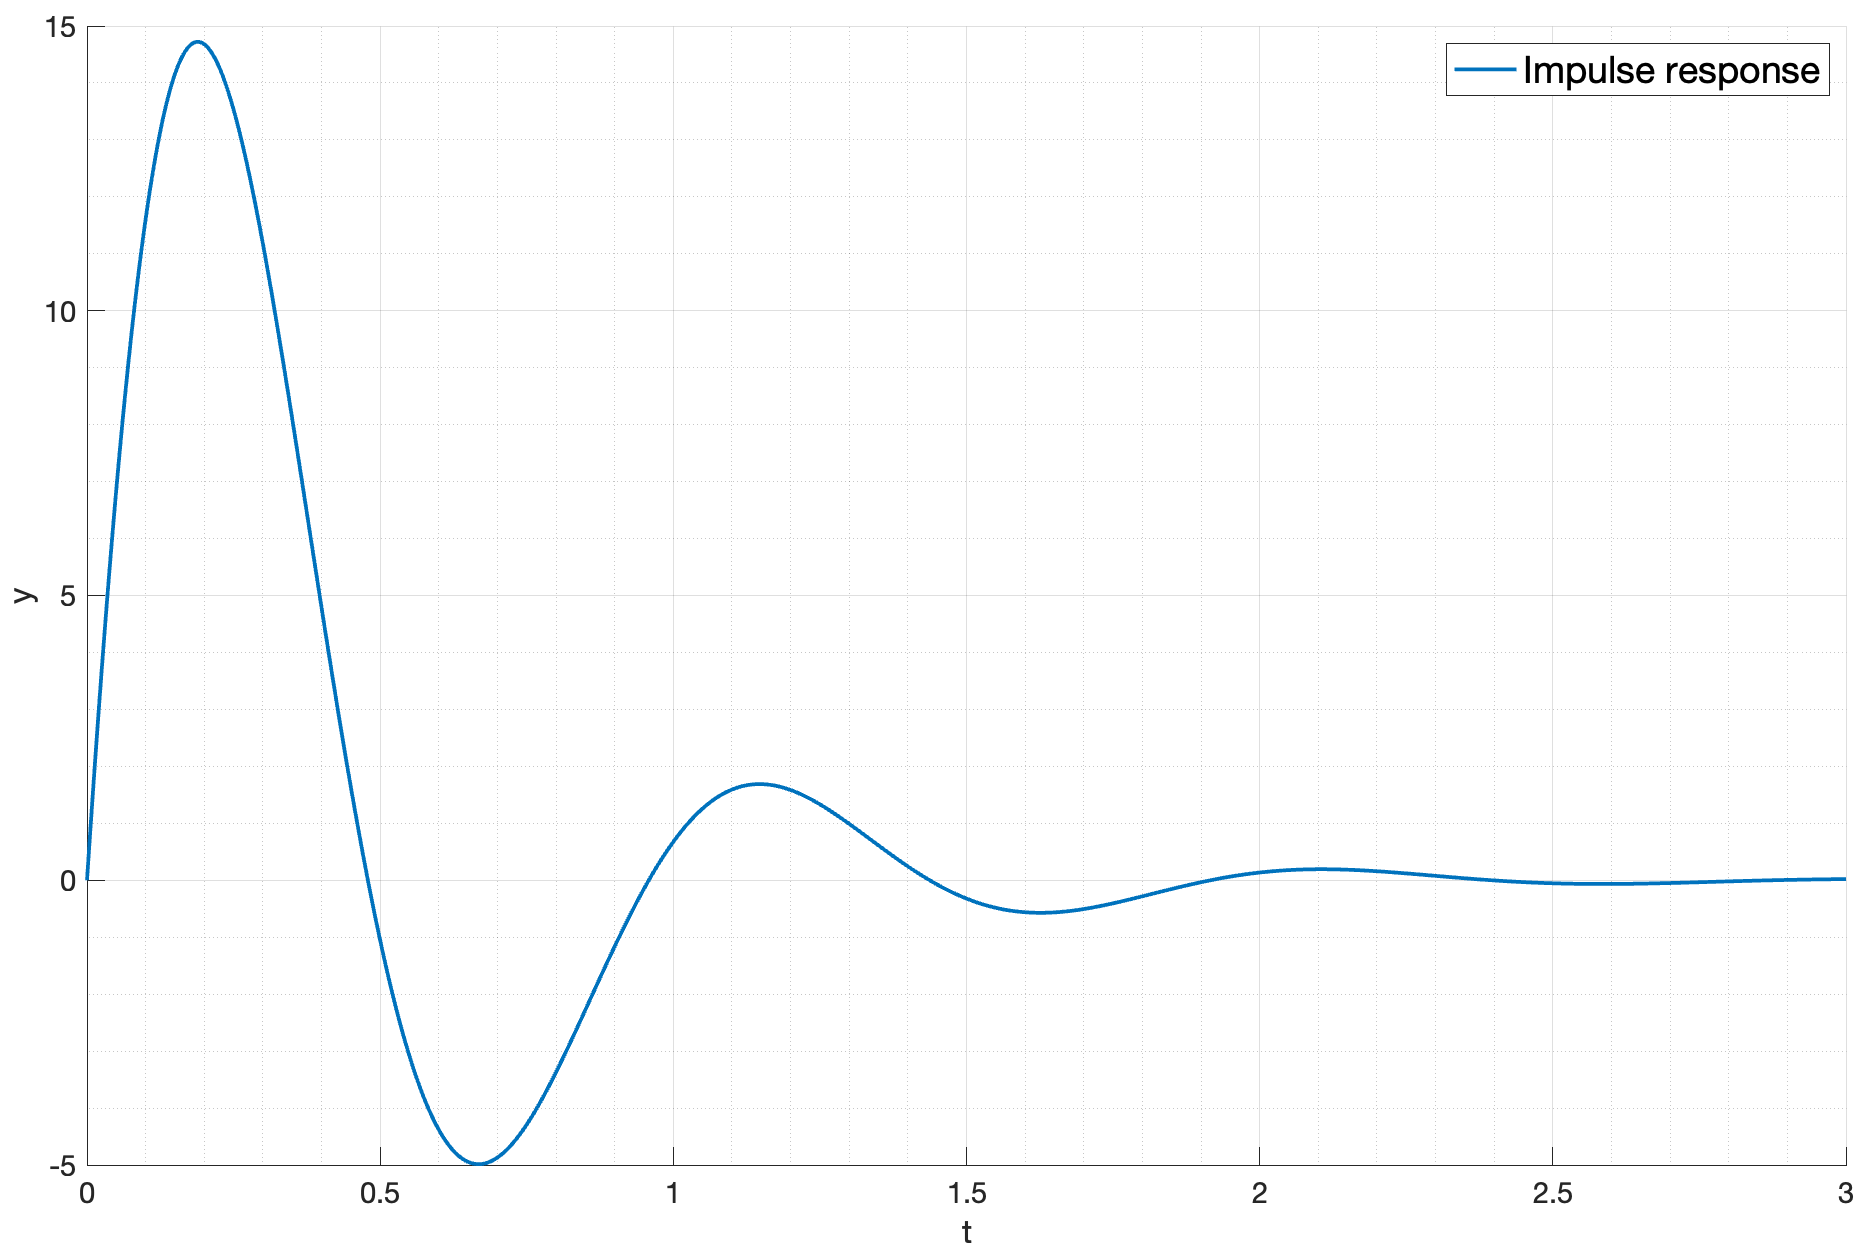
\includegraphics[width=\textwidth]{media/plots/task2_impulse_response_eq.png}
    \caption{Весовая функция двигателя постоянного тока 2.0 (теоретически)}
    \label{fig:task2_impulse_response_eq}
\end{figure}
\begin{figure}[ht!]
    \centering
    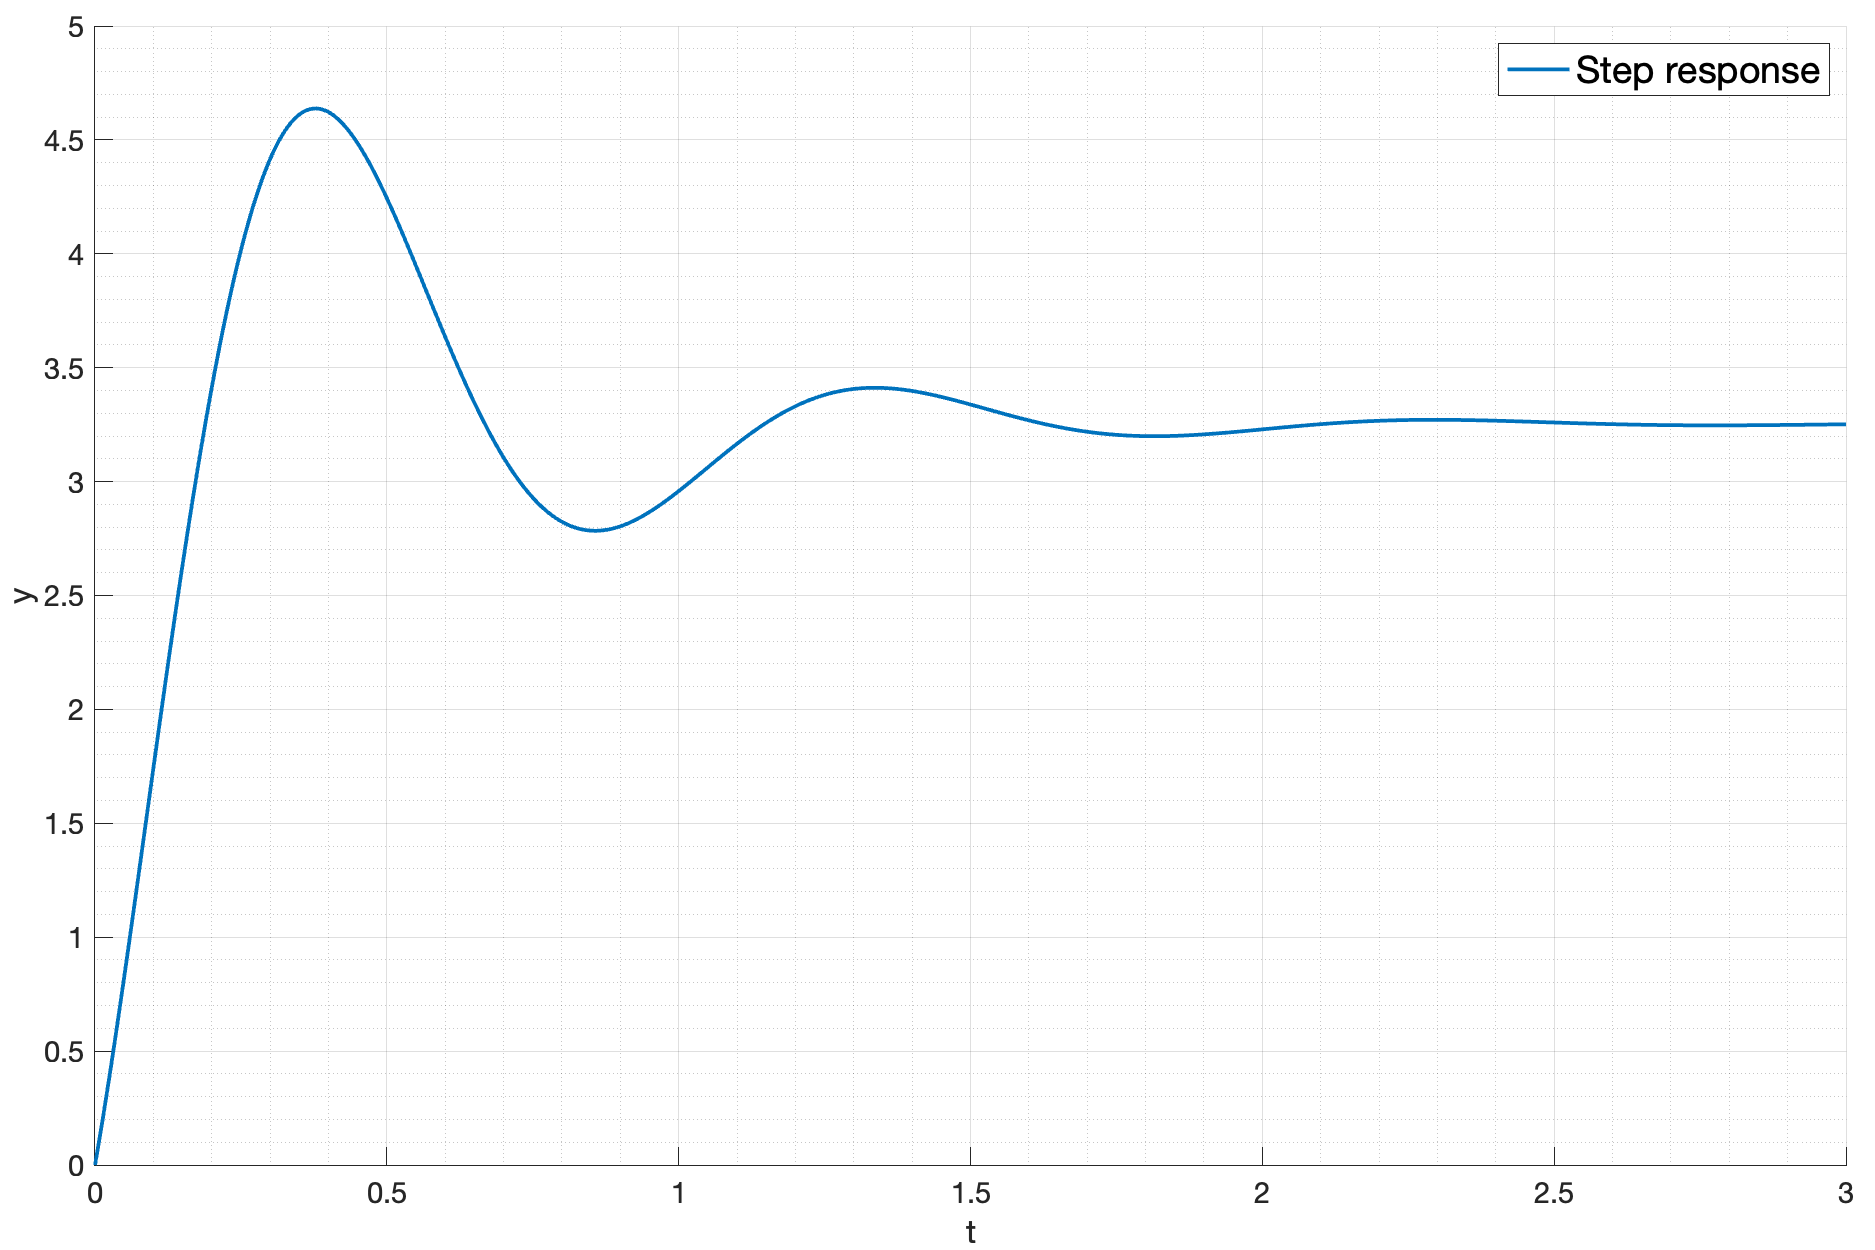
\includegraphics[width=\textwidth]{media/plots/task2_step_response_eq.png}
    \caption{Переходная функция двигателя постоянного тока 2.0 (теоретически)}
    \label{fig:task2_step_response_eq}
\end{figure}

Весовая (см. рис. \ref{fig:task2_impulse_response_exp}) и переходная (см. рис. \ref{fig:task2_step_response_exp}) функции, полученные в результате моделирования:
\begin{figure}[ht!]
    \centering
    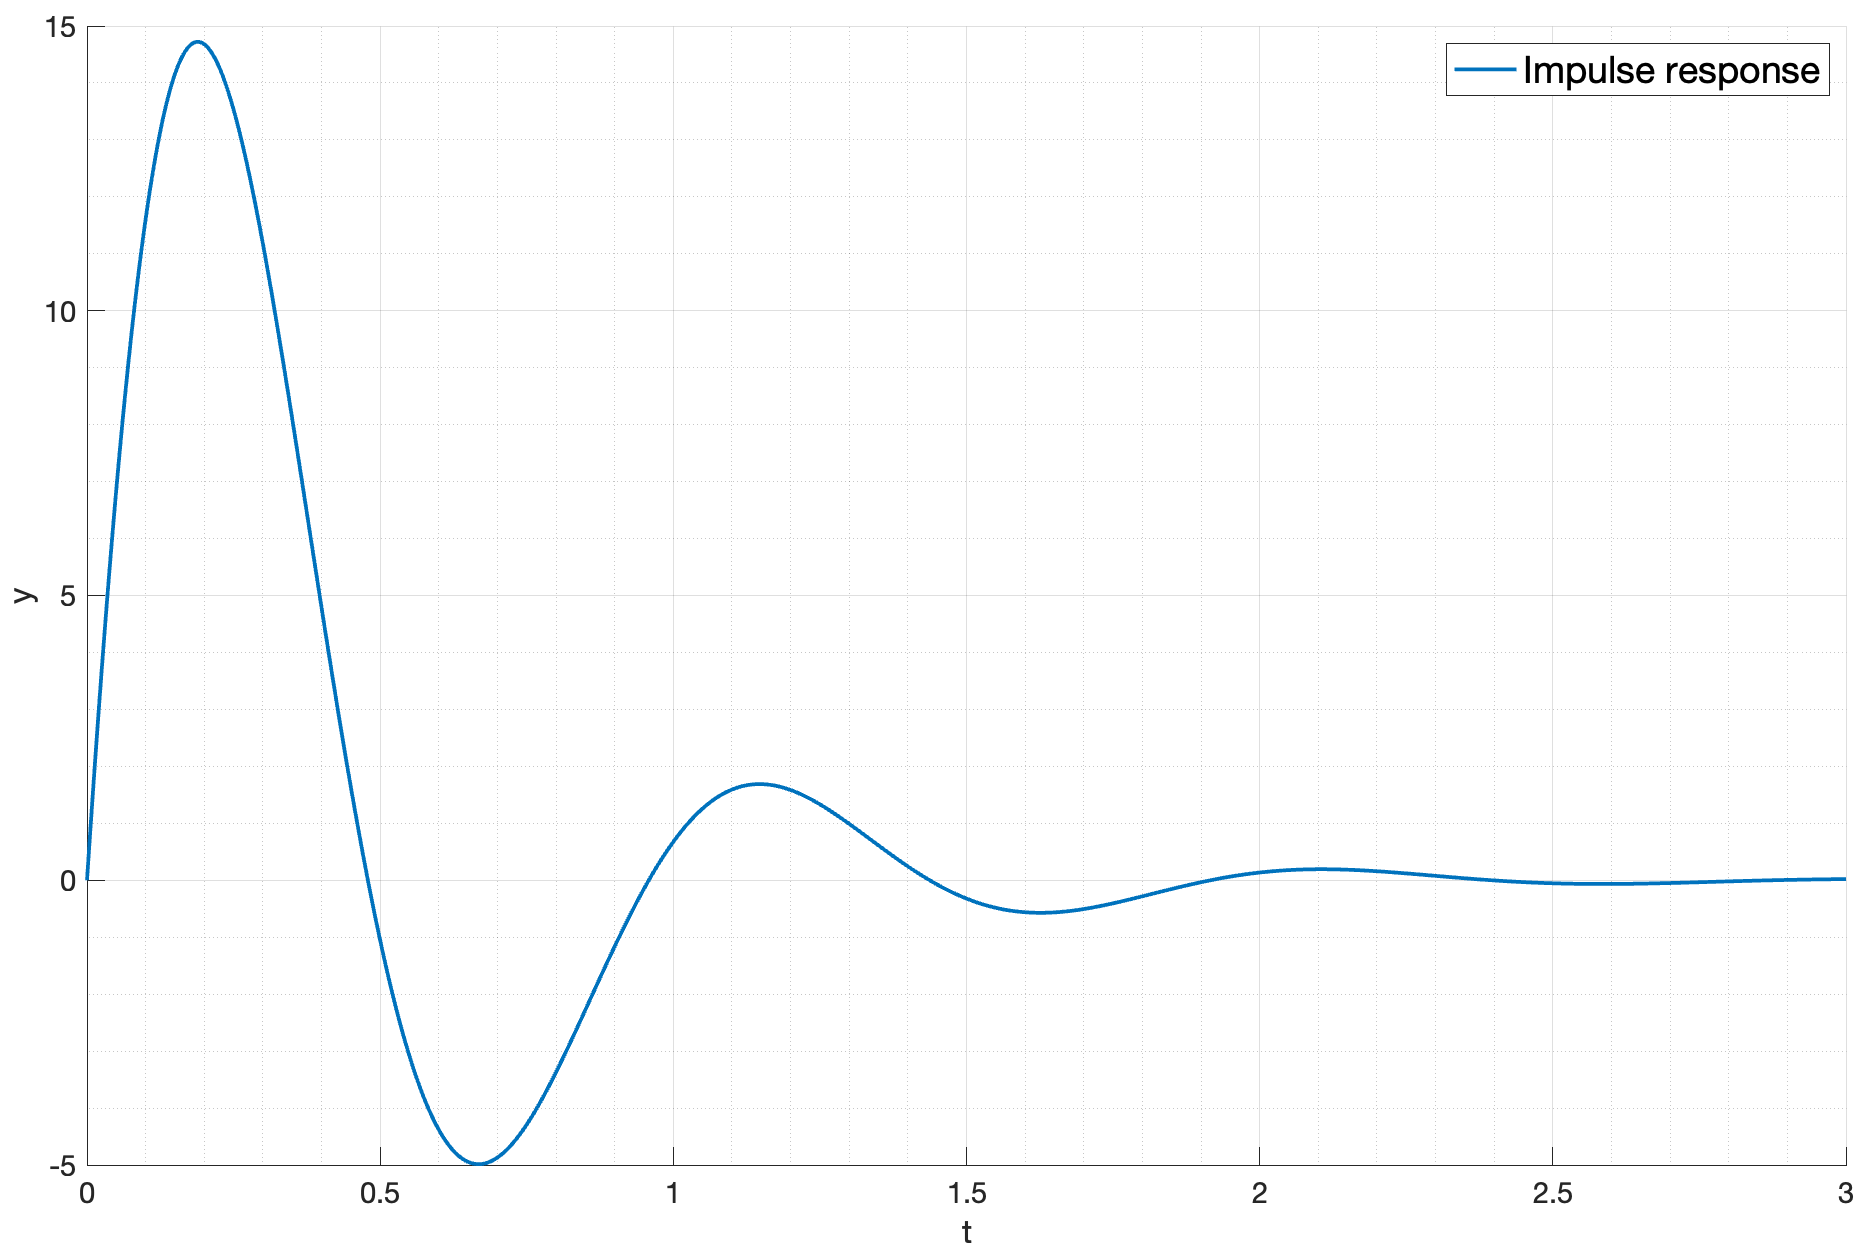
\includegraphics[width=\textwidth]{media/plots/task2_impulse_response_exp.png}
    \caption{Весовая функция двигателя постоянного тока 2.0 (экспериментально)}
    \label{fig:task2_impulse_response_exp}
\end{figure}
\begin{figure}[ht!]
    \centering
    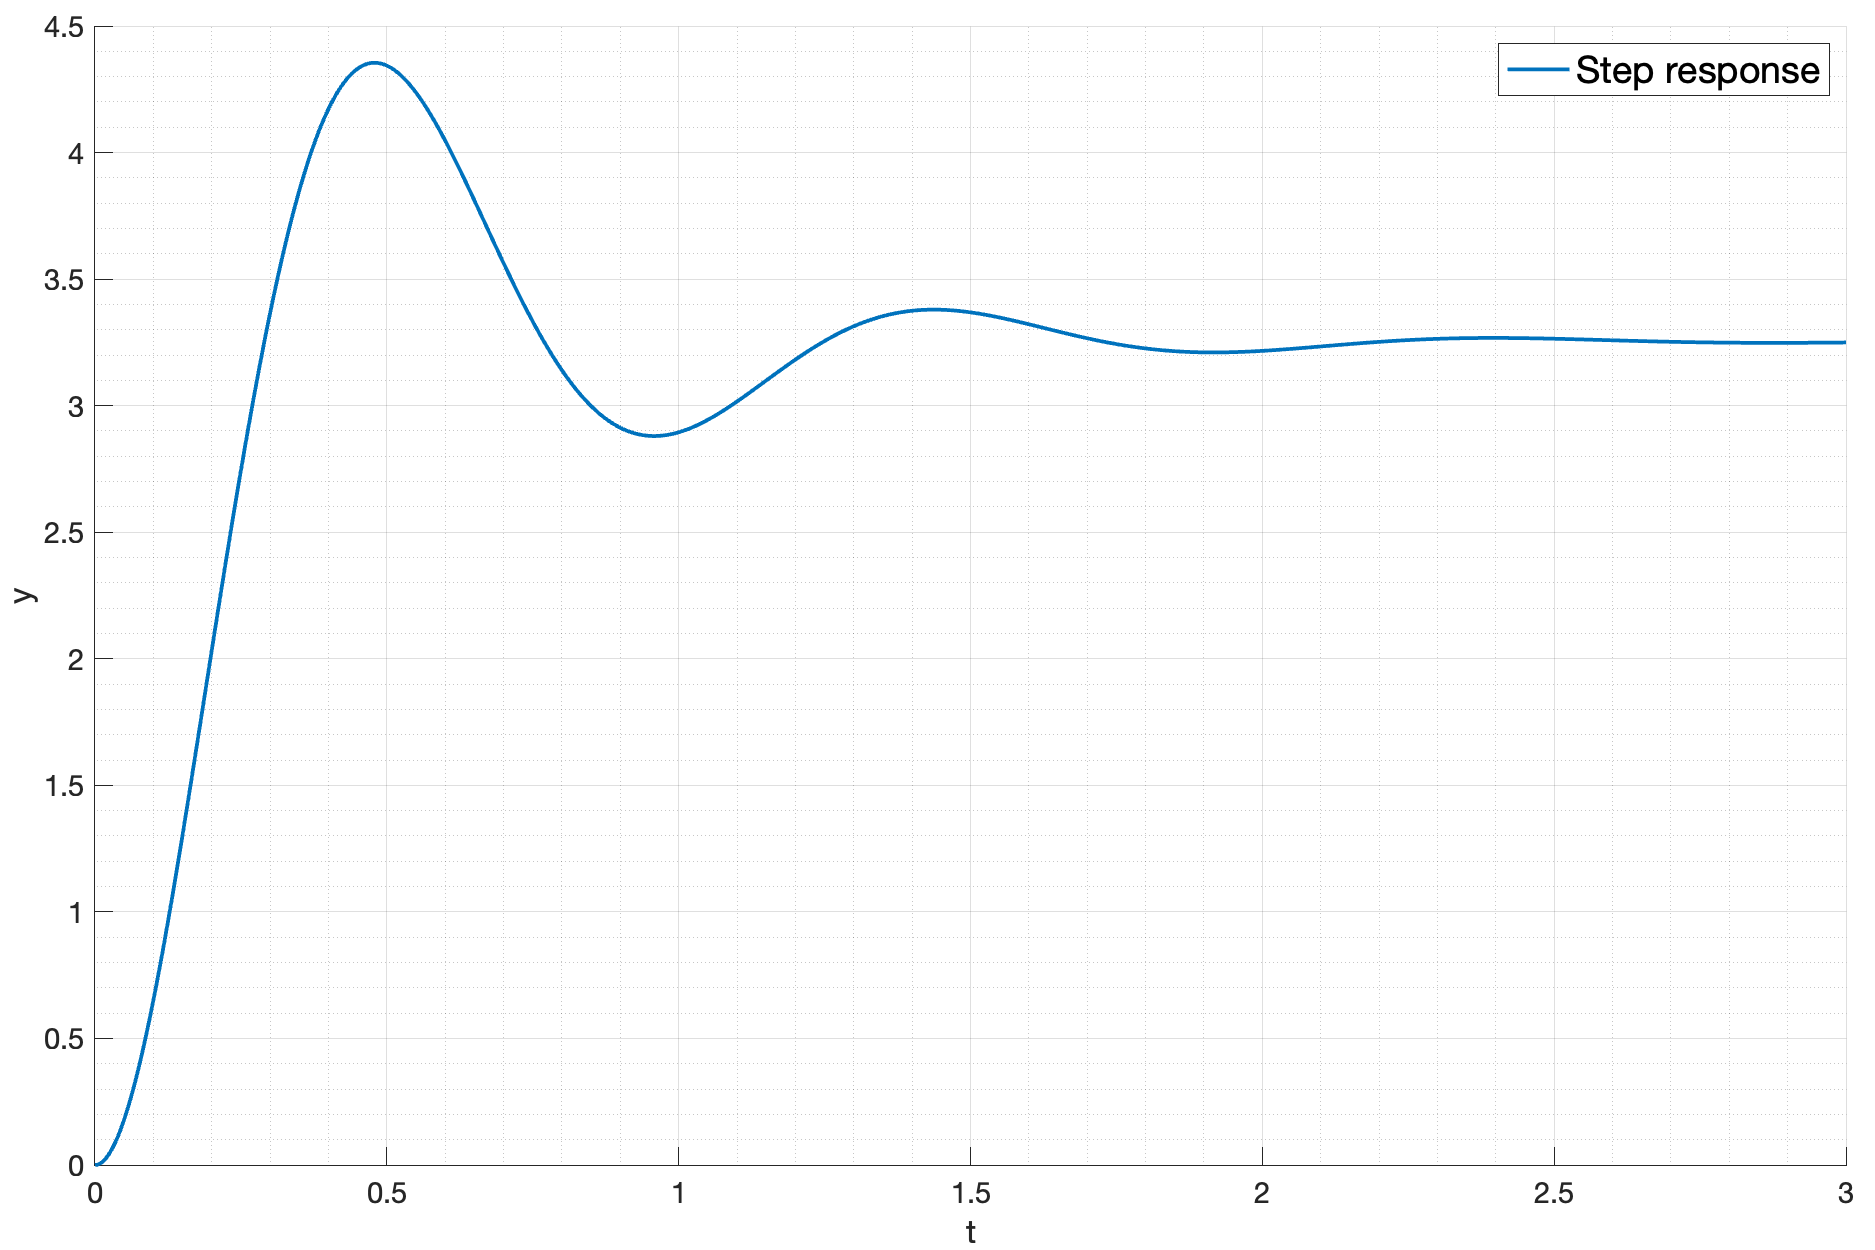
\includegraphics[width=\textwidth]{media/plots/task2_step_response_exp.png}
    \caption{Переходная функция двигателя постоянного тока 2.0 (экспериментально)}
    \label{fig:task2_step_response_exp}
\end{figure}

Сравнительные графики приведены на рис. \ref{fig:task2_impulse_response_cmp} и рис. \ref{fig:task2_step_response_cmp}.
\begin{figure}[ht!]
    \centering
    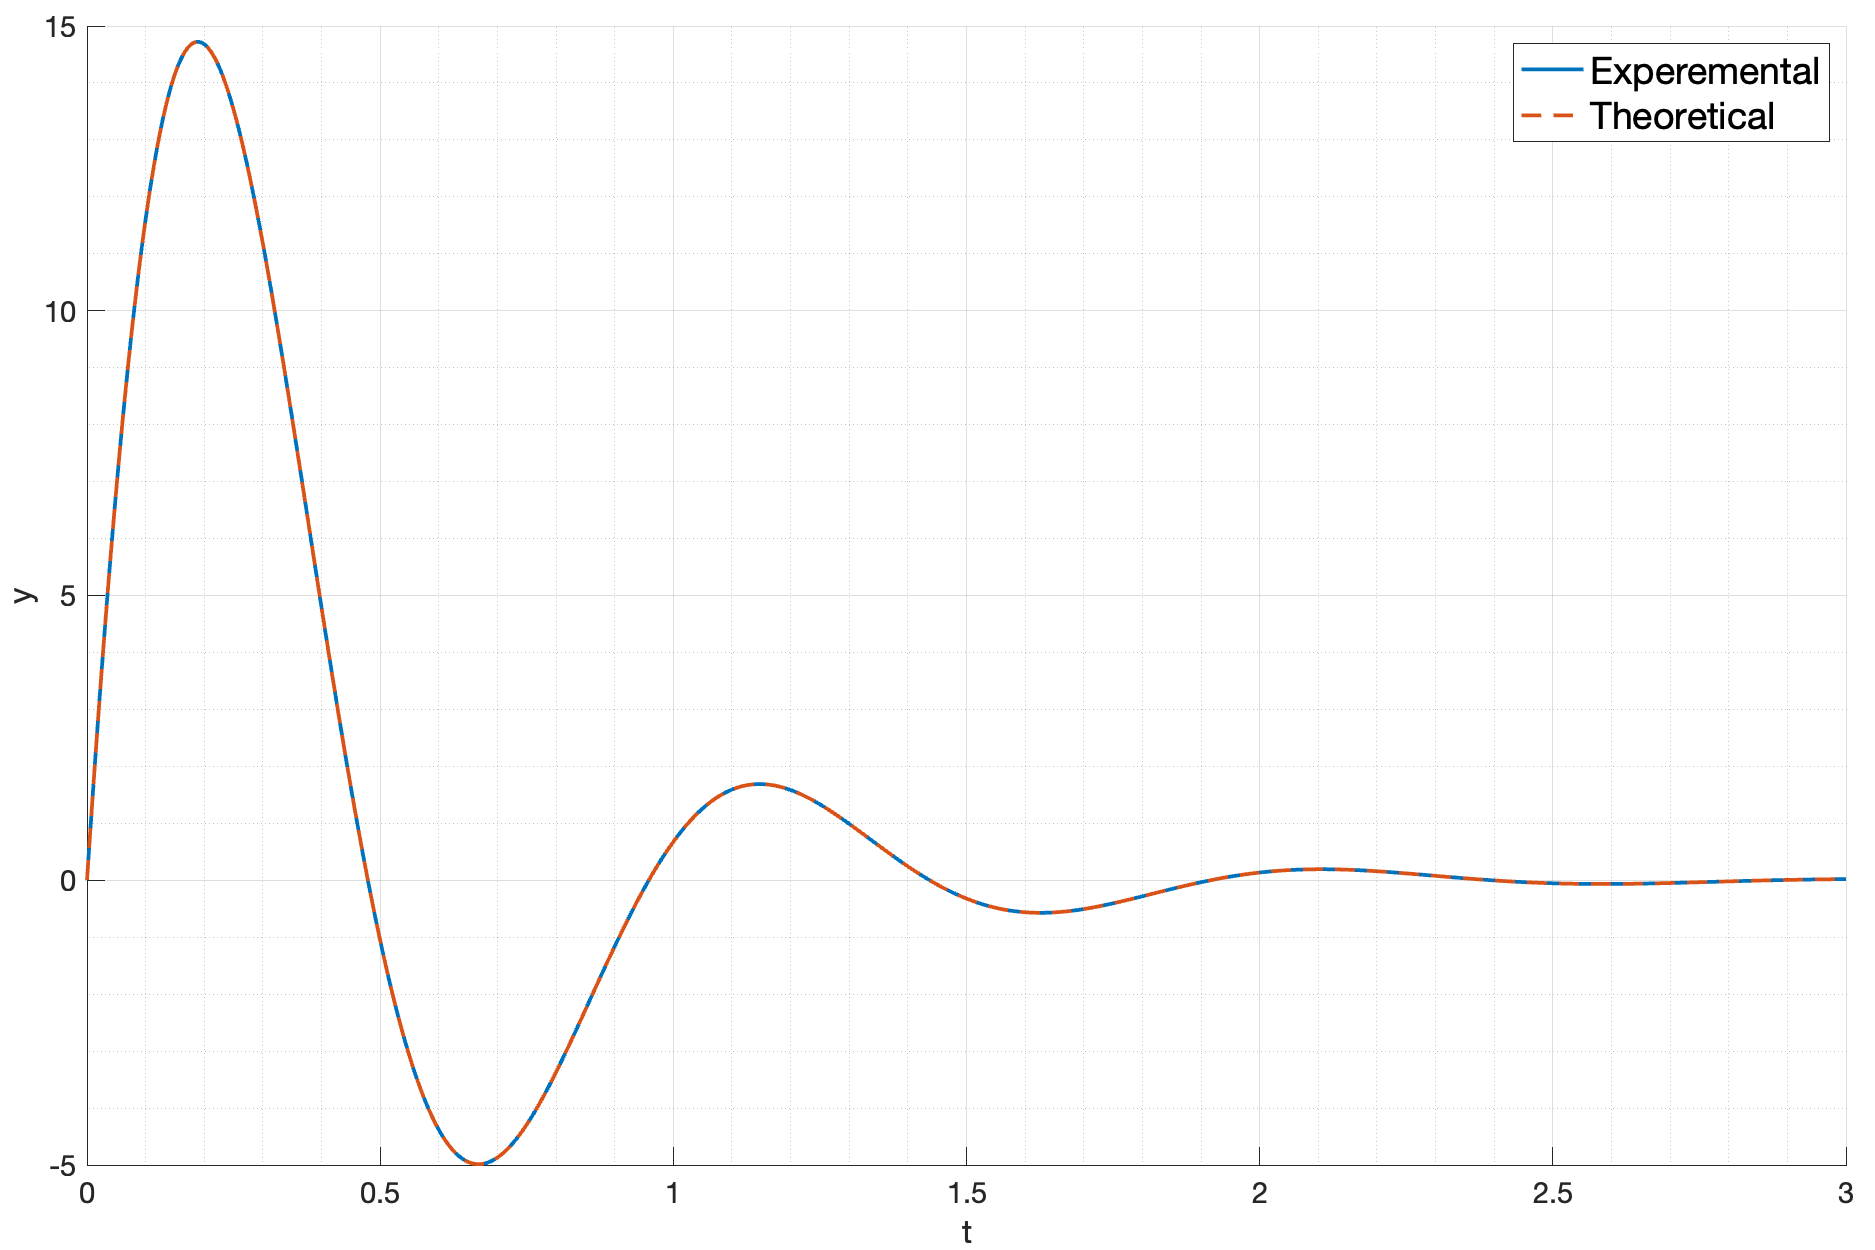
\includegraphics[width=\textwidth]{media/plots/task2_impulse_response_cmp.png}
    \caption{Сравнение весовых функций двигателя постоянного тока 2.0}
    \label{fig:task2_impulse_response_cmp}
\end{figure}
\begin{figure}[ht!]
    \centering
    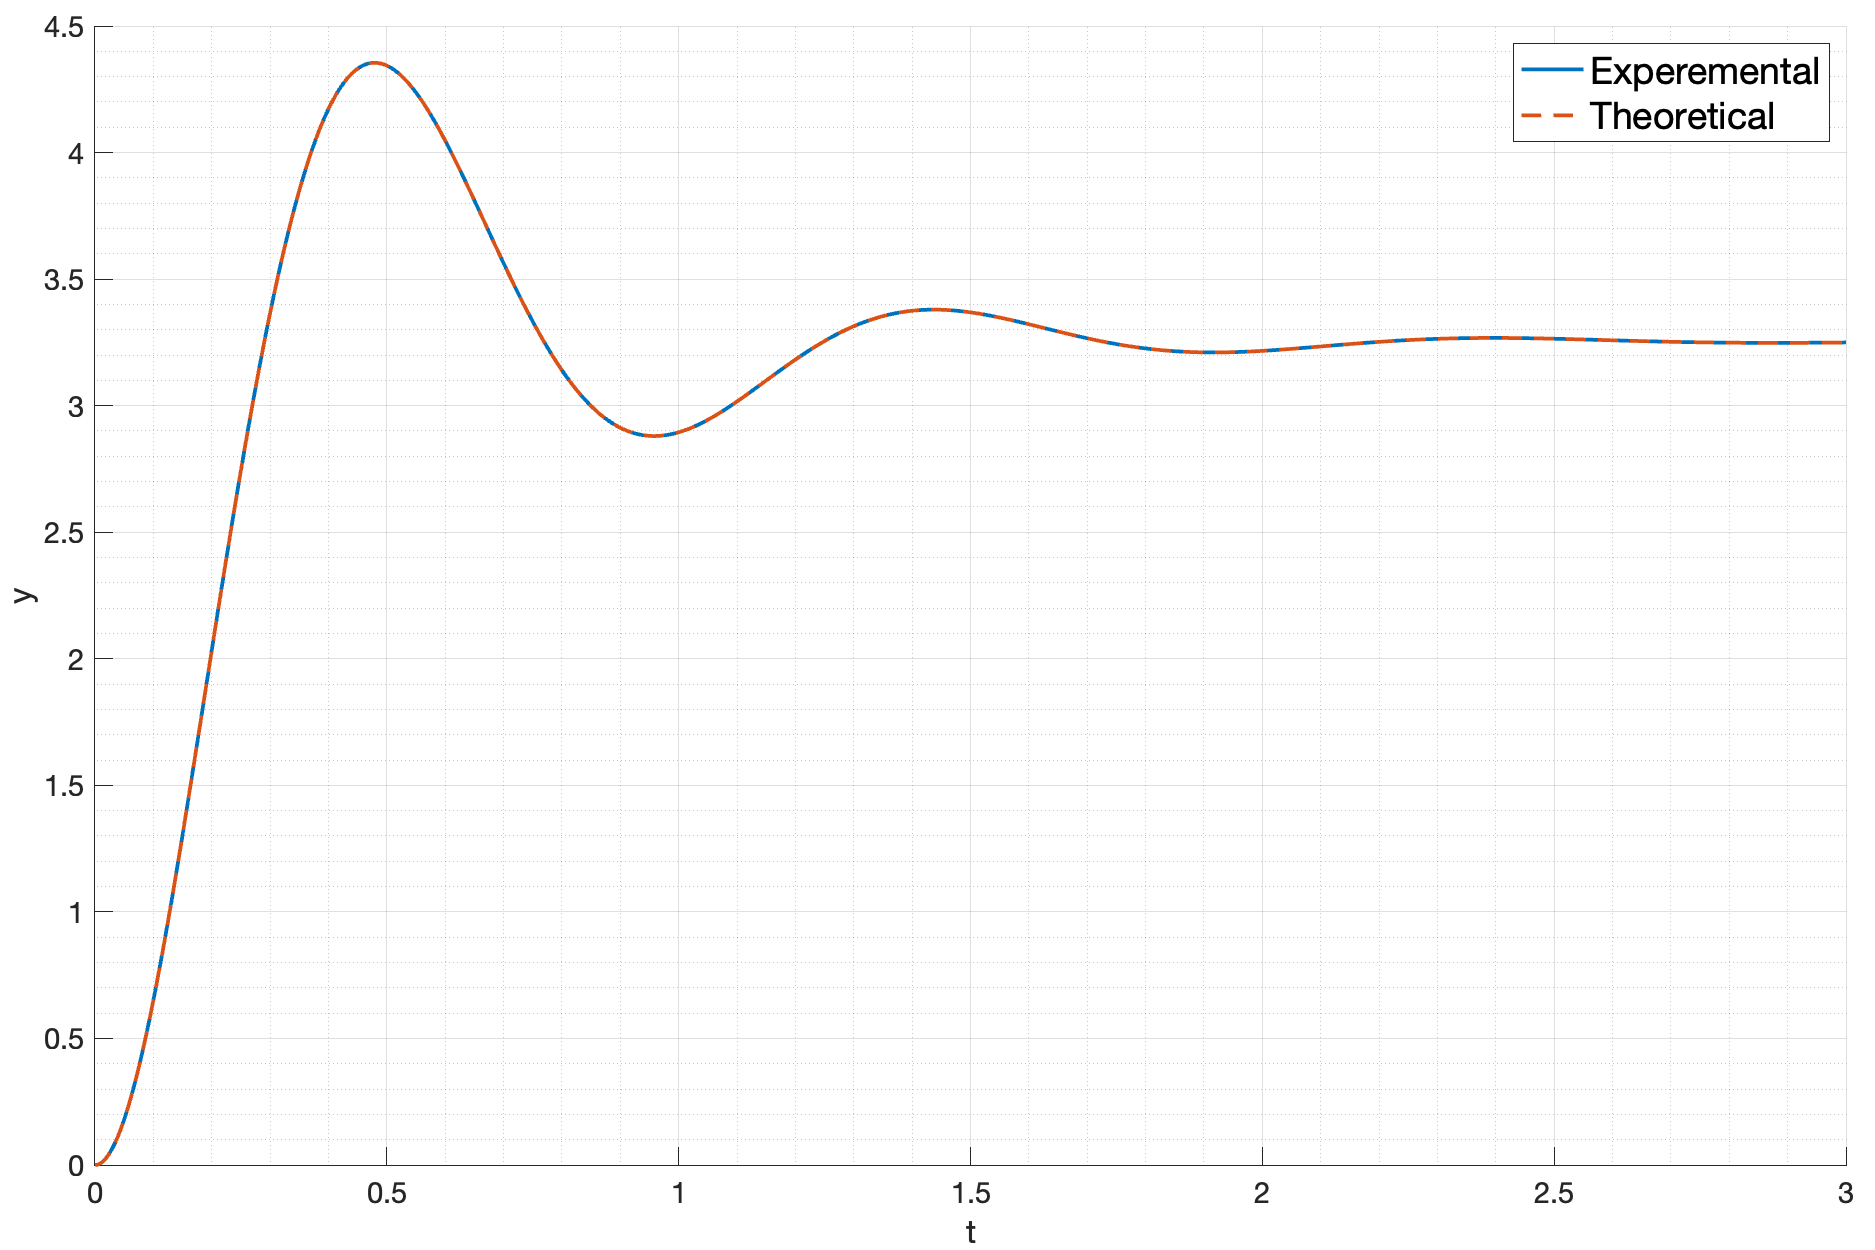
\includegraphics[width=\textwidth]{media/plots/task2_step_response_cmp.png}
    \caption{Сравнение переходных функций двигателя постоянного тока 2.0}
    \label{fig:task2_step_response_cmp}
\end{figure}

\FloatBarrier
\subsection{Частотные характеристики}
Найдем АЧХ и ФЧХ системы. Для этого подставим $s = j\omega$ в передаточную функцию:
\begin{eqnarray}
    W(j\omega) =  \frac{1/k_e}{T^2j^2\omega^2 + 2\beta Tj\omega + 1} = \frac{1/k_e(1 - T^2\omega^2)}{(1 - T^2\omega^2) + (2T\beta\omega)^2} + \frac{-2\beta T\omega/k_e}{(1 - T^2\omega^2) + (2T\beta\omega)^2}
\end{eqnarray}
Амплитудная характеристика:
\begin{equation}
    A = \frac{1/k_e}{\sqrt{(1 - T^2\omega^2)^2 + (2T\beta\omega)^2}}
\end{equation}
Фазовая характеристика:
\begin{eqnarray}
    \varphi = -\text{atan2}\left(2T\beta\omega,~1 - T^2\omega^2\right)
\end{eqnarray}

Построим графики АЧХ, ФЧХ (см. рис. \ref{fig:task2_freq_resp_eq_lin}) и логарифмическую АЧХ (см. рис. \ref{fig:task2_freq_resp_eq_loglog}).

\begin{figure}[ht!]
    \centering
    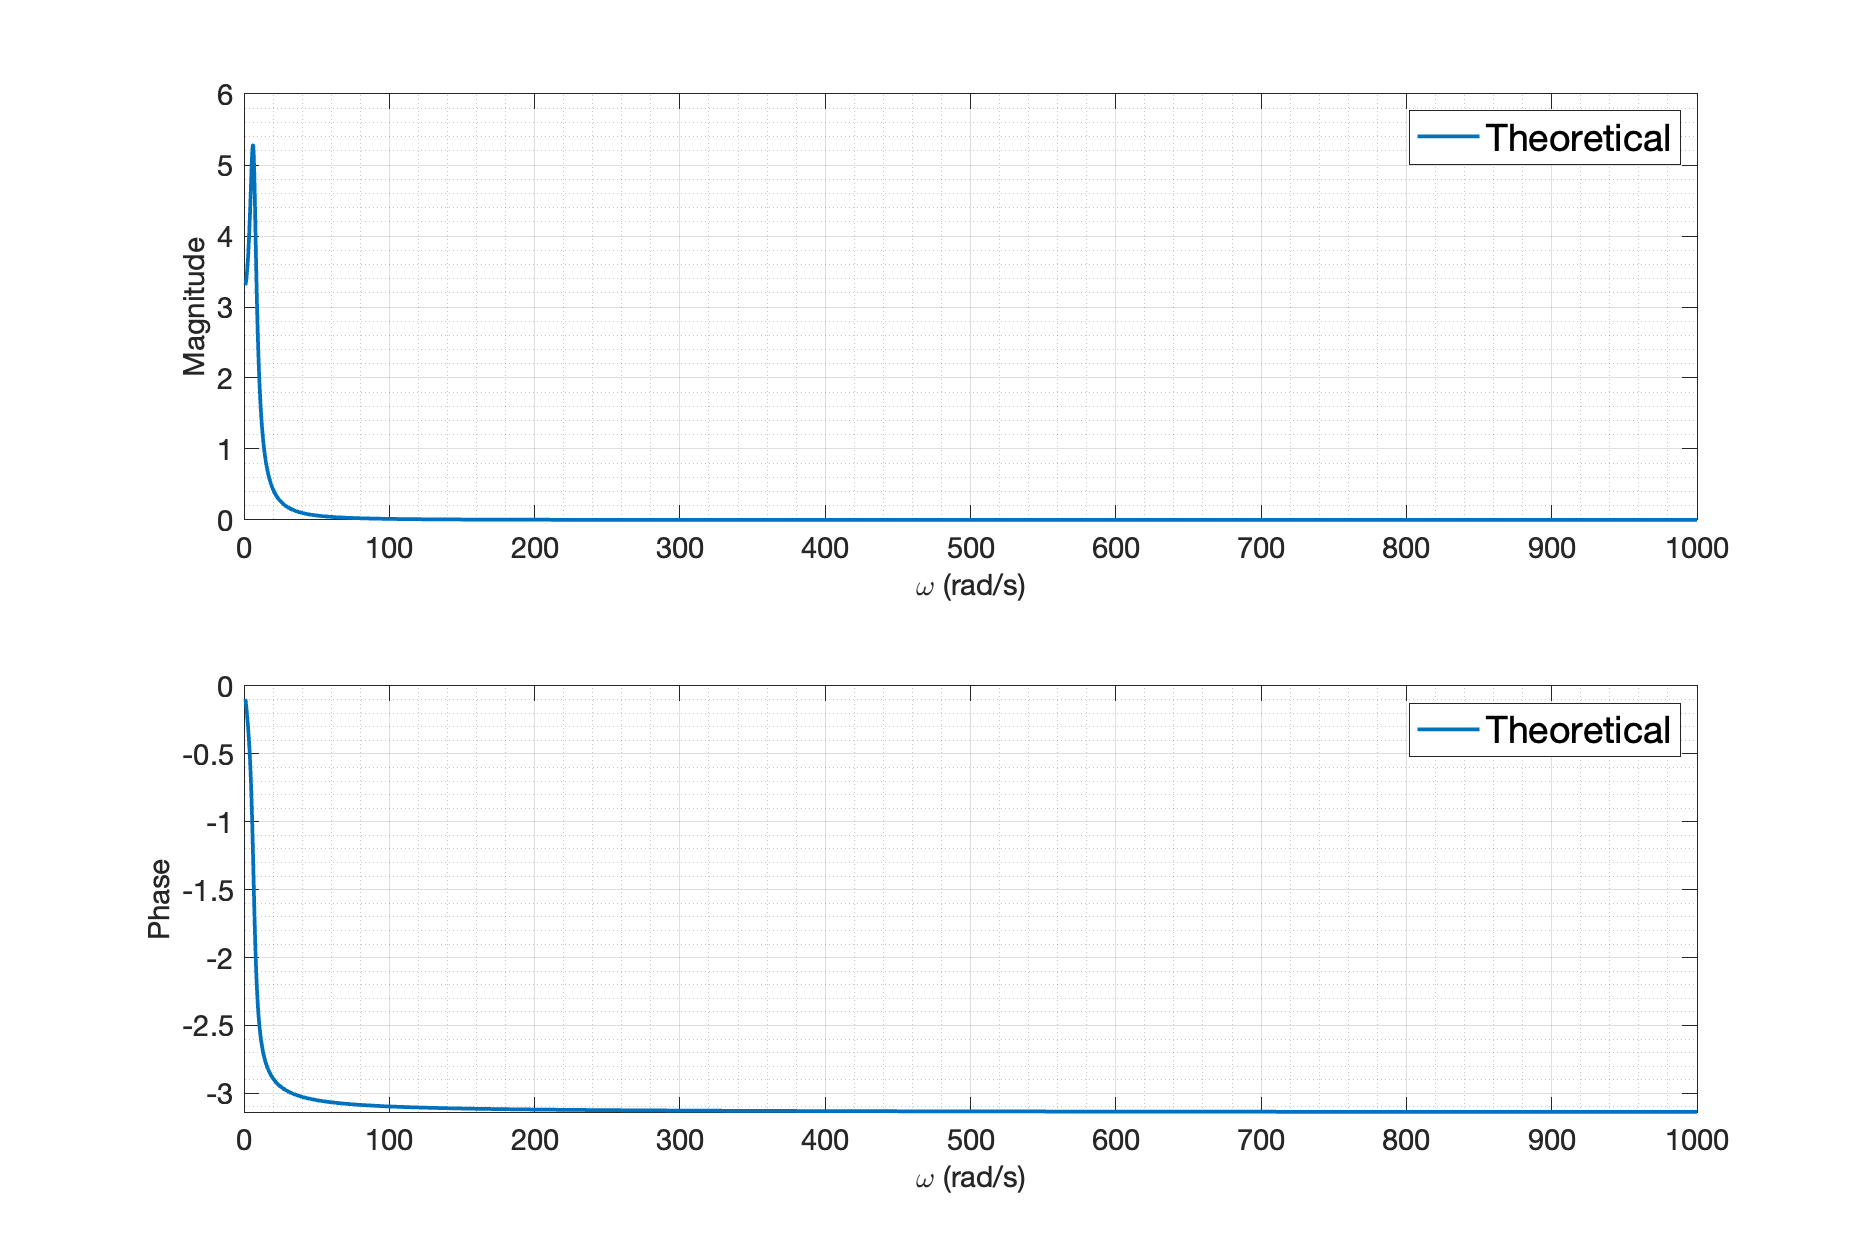
\includegraphics[width=\textwidth]{media/plots/task2_freq_resp_eq_lin.png}
    \caption{АЧХ и ФЧХ двигателя постоянного тока 2.0 (теоретически)}
    \label{fig:task2_freq_resp_eq_lin}
\end{figure}
\begin{figure}[ht!]
    \centering
    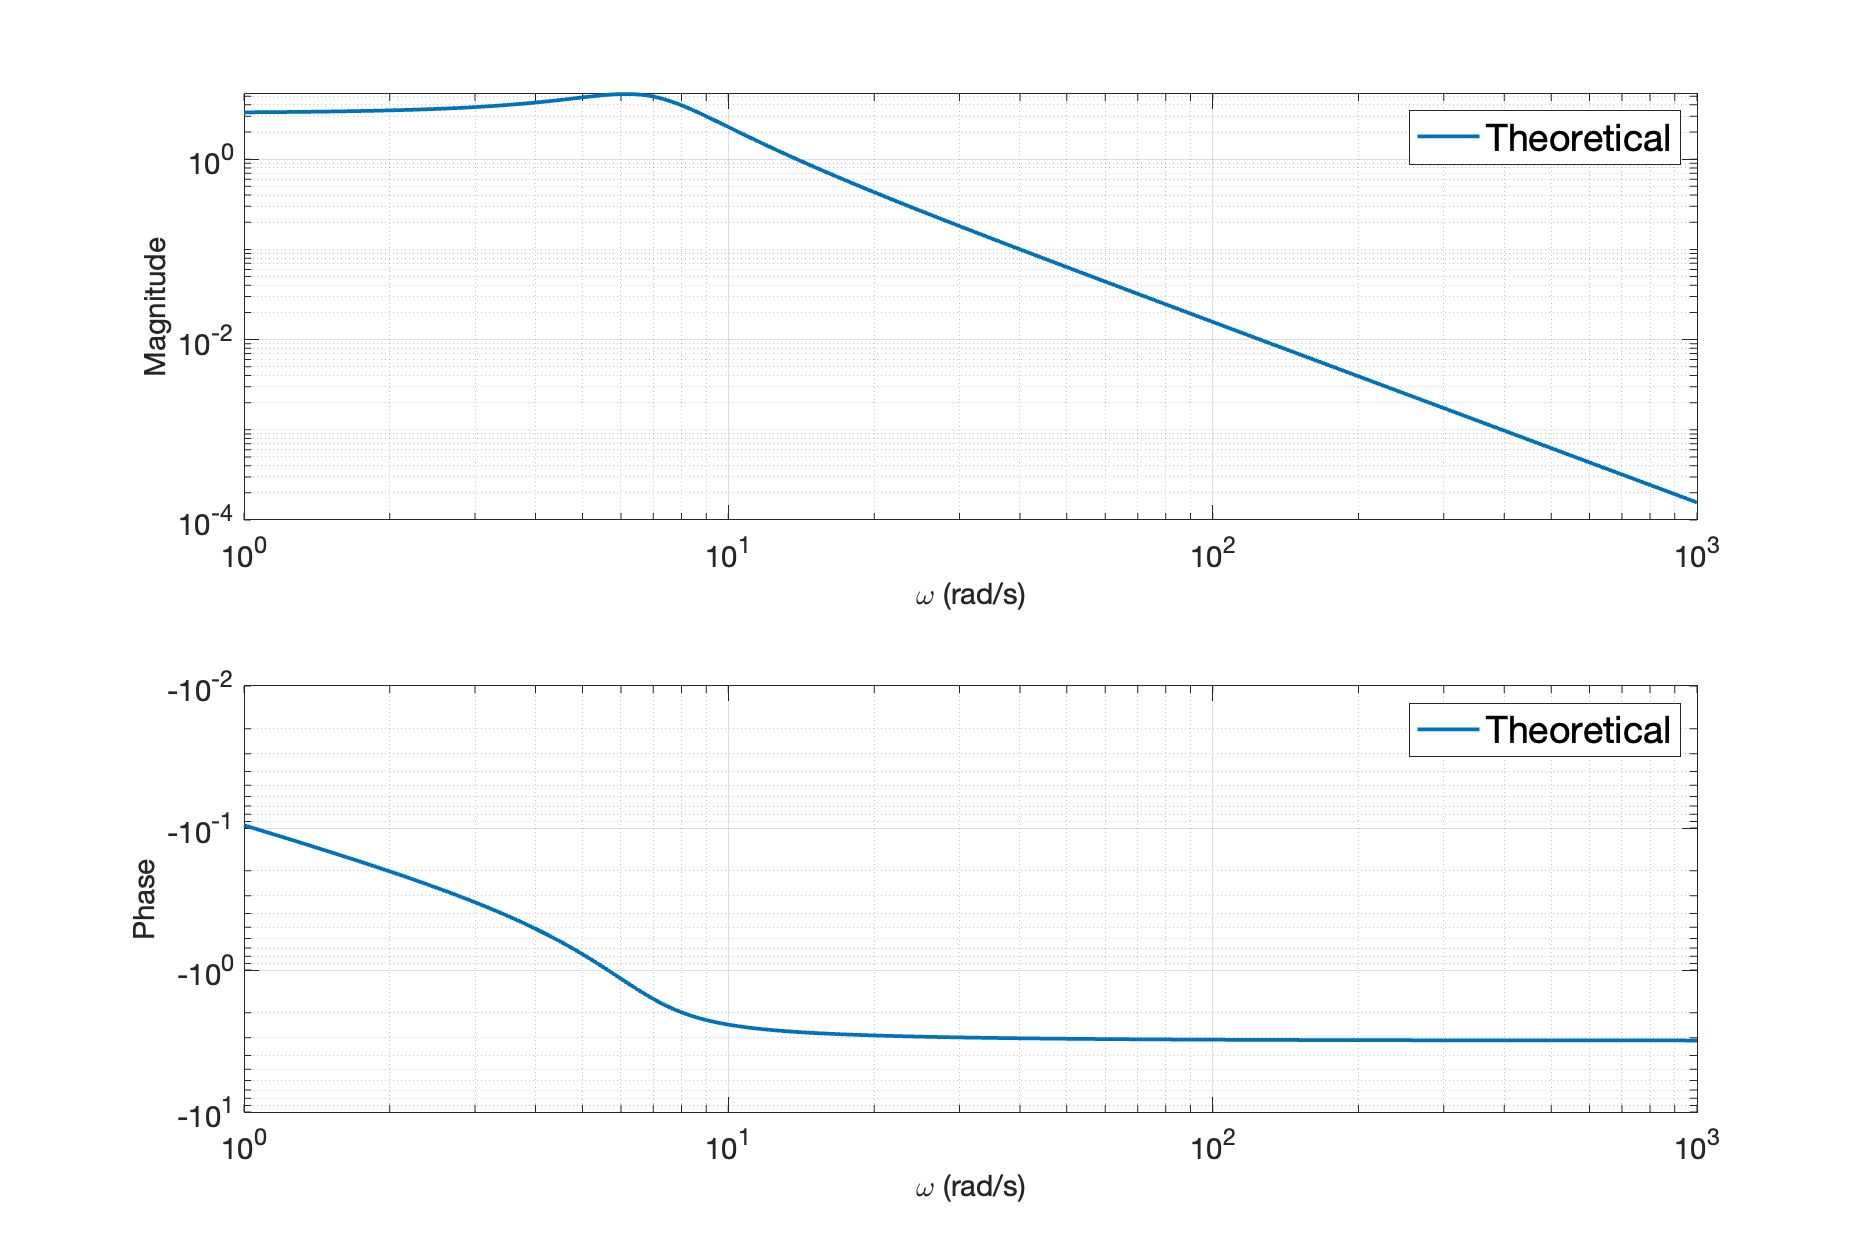
\includegraphics[width=\textwidth]{media/plots/task2_freq_resp_eq_loglog.png}
    \caption{Логарифмическая АЧХ двигателя постоянного тока 2.0 (теоретически)}
    \label{fig:task2_freq_resp_eq_loglog}
\end{figure}

AЧХ, ФЧХ и логарифмическая АЧХ, полученные в результате моделирования приведены на рис. \ref{fig:task2_freq_resp_exp_lin} и рис. \ref{fig:task2_freq_resp_exp_loglog}.
\begin{figure}[ht!]
    \centering
    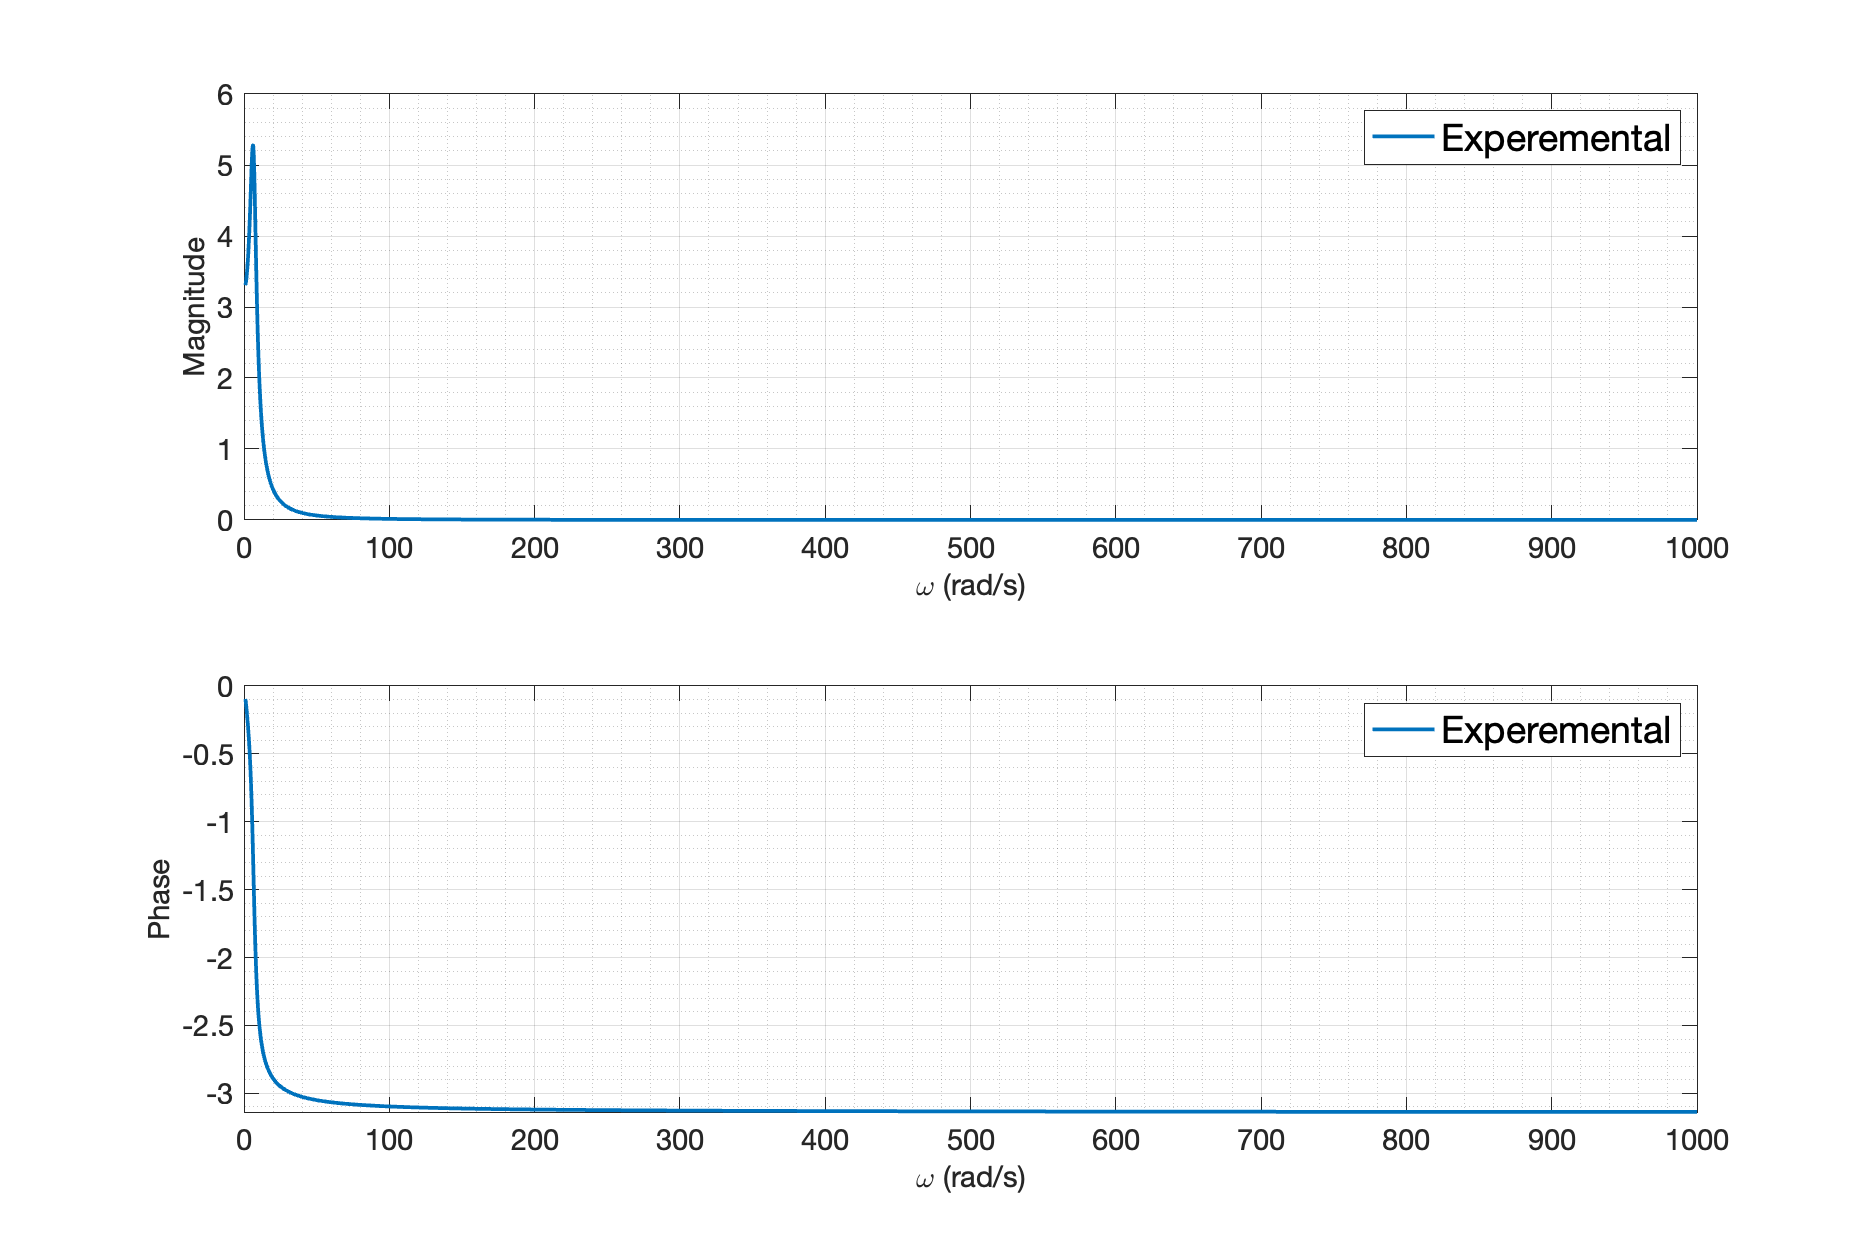
\includegraphics[width=\textwidth]{media/plots/task2_freq_resp_exp_lin.png}
    \caption{АЧХ и ФЧХ двигателя постоянного тока 2.0 (экспериментально)}
    \label{fig:task2_freq_resp_exp_lin}
\end{figure}
\begin{figure}[ht!]
    \centering
    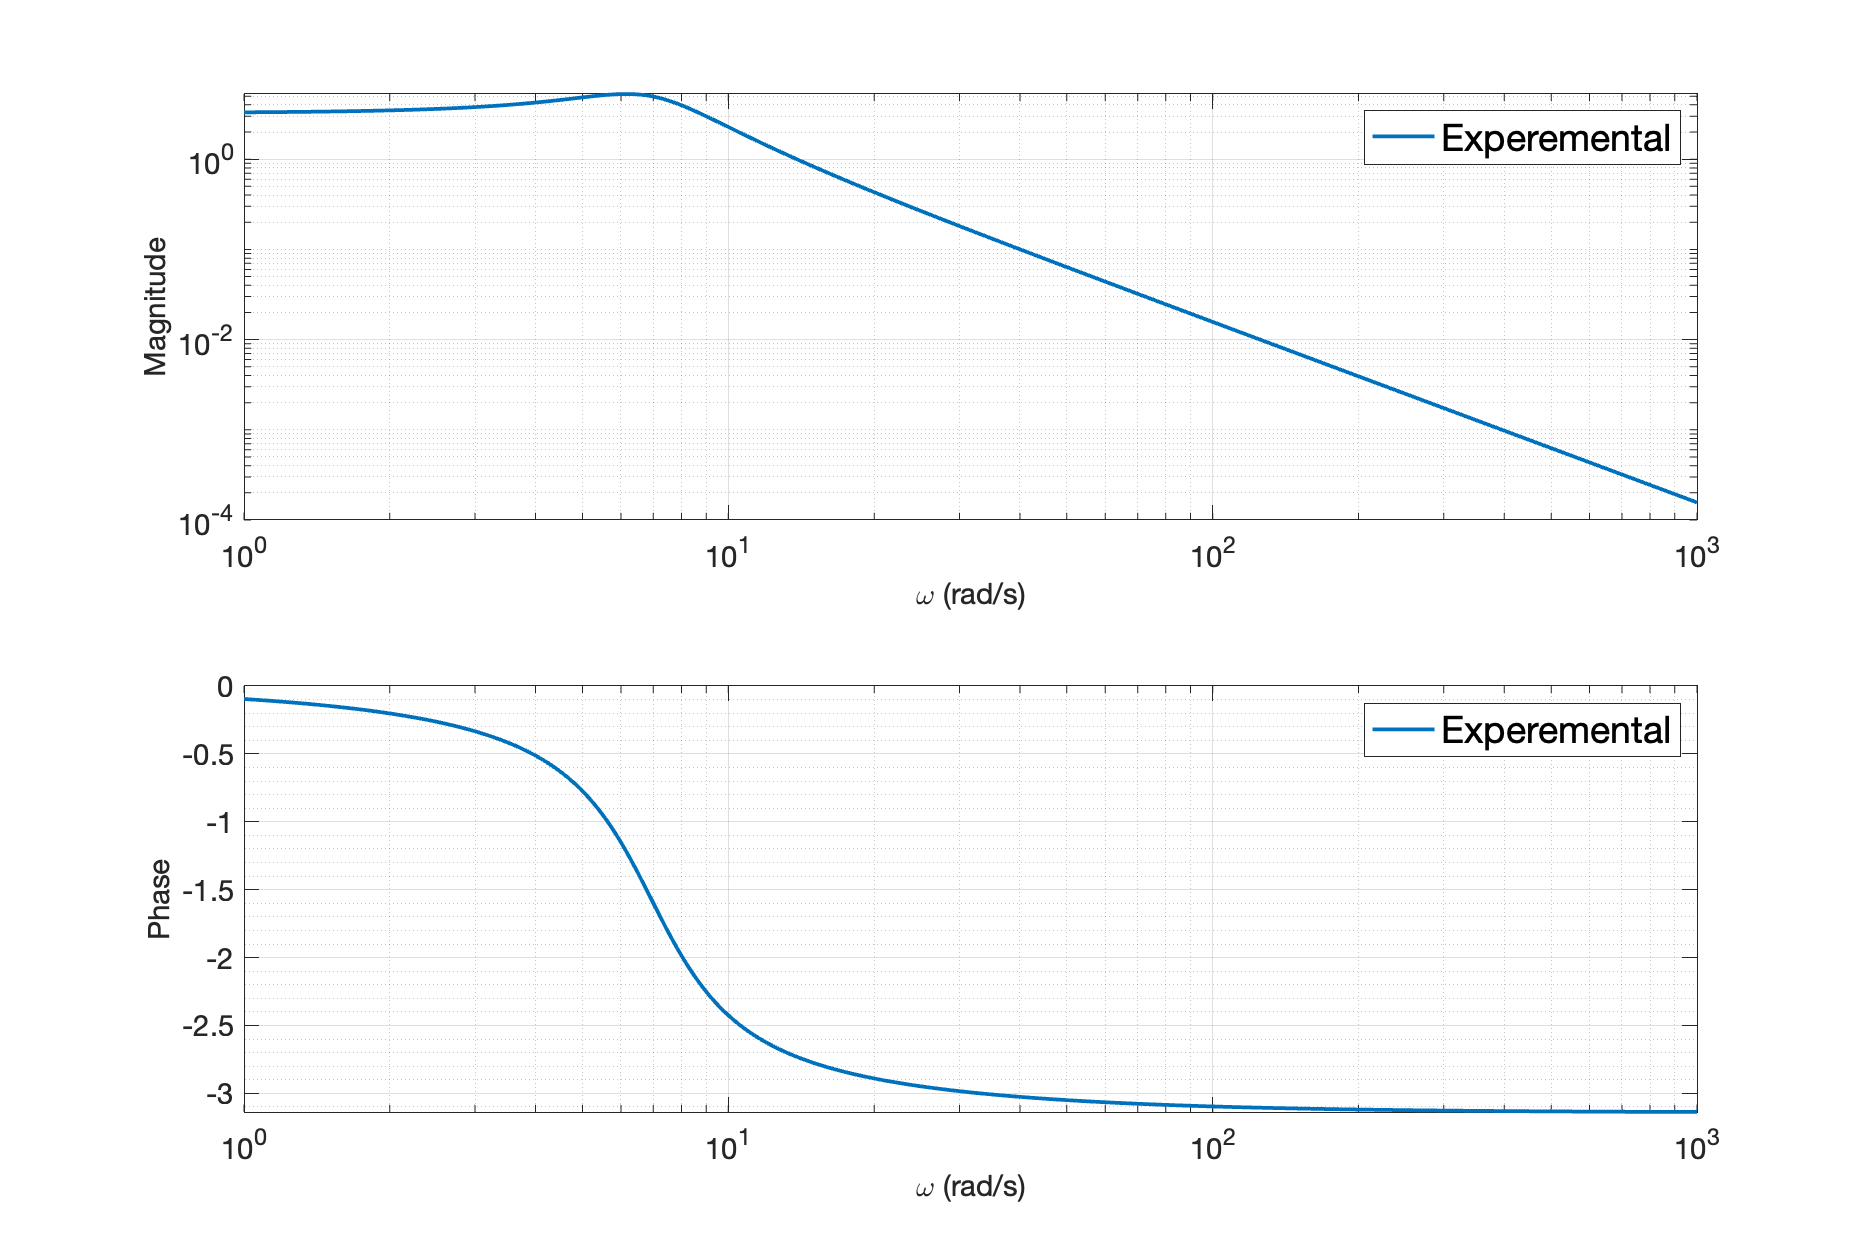
\includegraphics[width=\textwidth]{media/plots/task2_freq_resp_exp_loglog.png}
    \caption{Логарифмическая АЧХ двигателя постоянного тока 2.0 (экспериментально)}
    \label{fig:task2_freq_resp_exp_loglog}
\end{figure}

Сравнительные графики приведены на рис. \ref{fig:task2_freq_resp_cmp_lin} и рис. \ref{fig:task2_freq_resp_cmp_loglog}.
\begin{figure}[ht!]
    \centering
    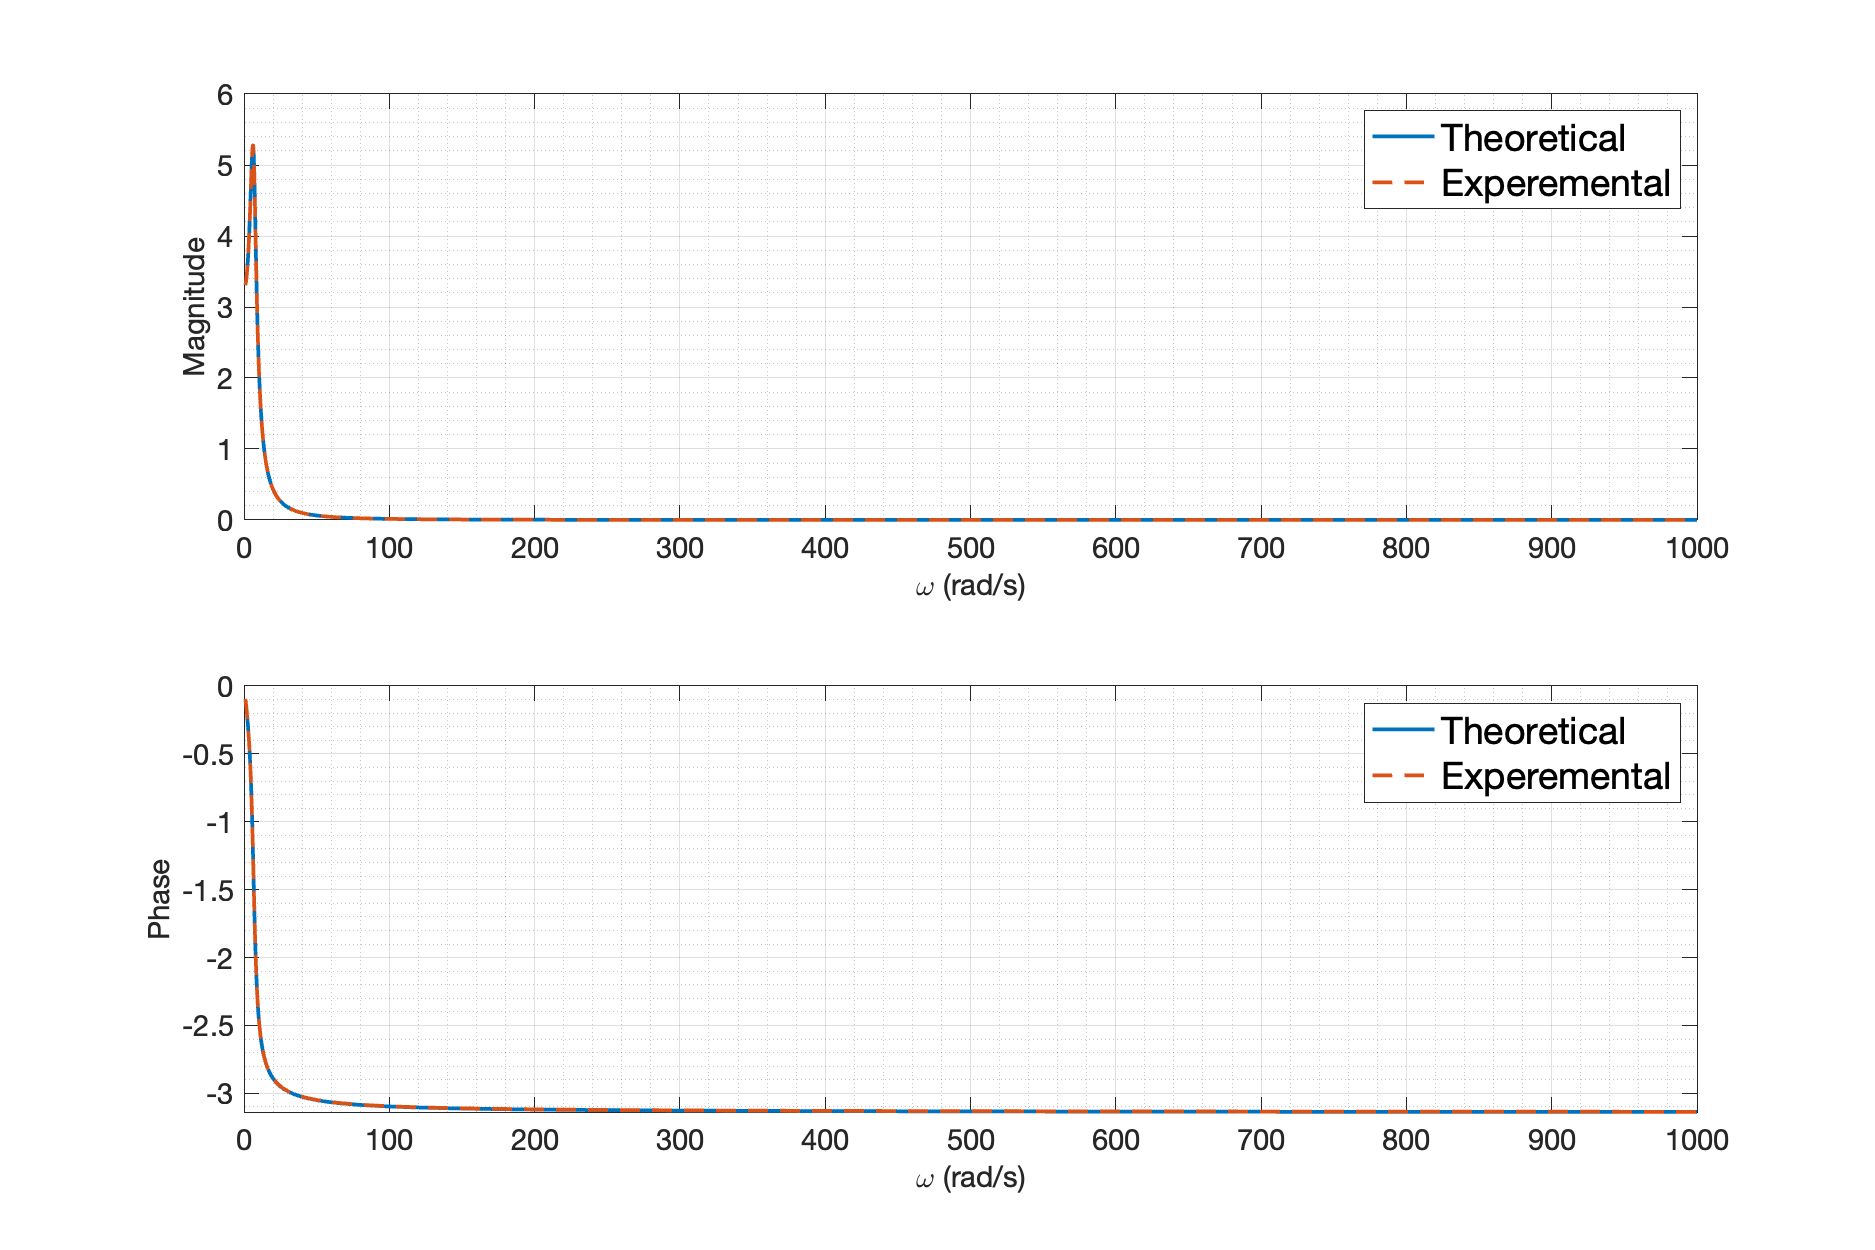
\includegraphics[width=\textwidth]{media/plots/task2_freq_resp_cmp_lin.png}
    \caption{Сравнение АЧХ и ФЧХ двигателя постоянного тока 2.0}
    \label{fig:task2_freq_resp_cmp_lin}
\end{figure}
\begin{figure}[ht!]
    \centering
    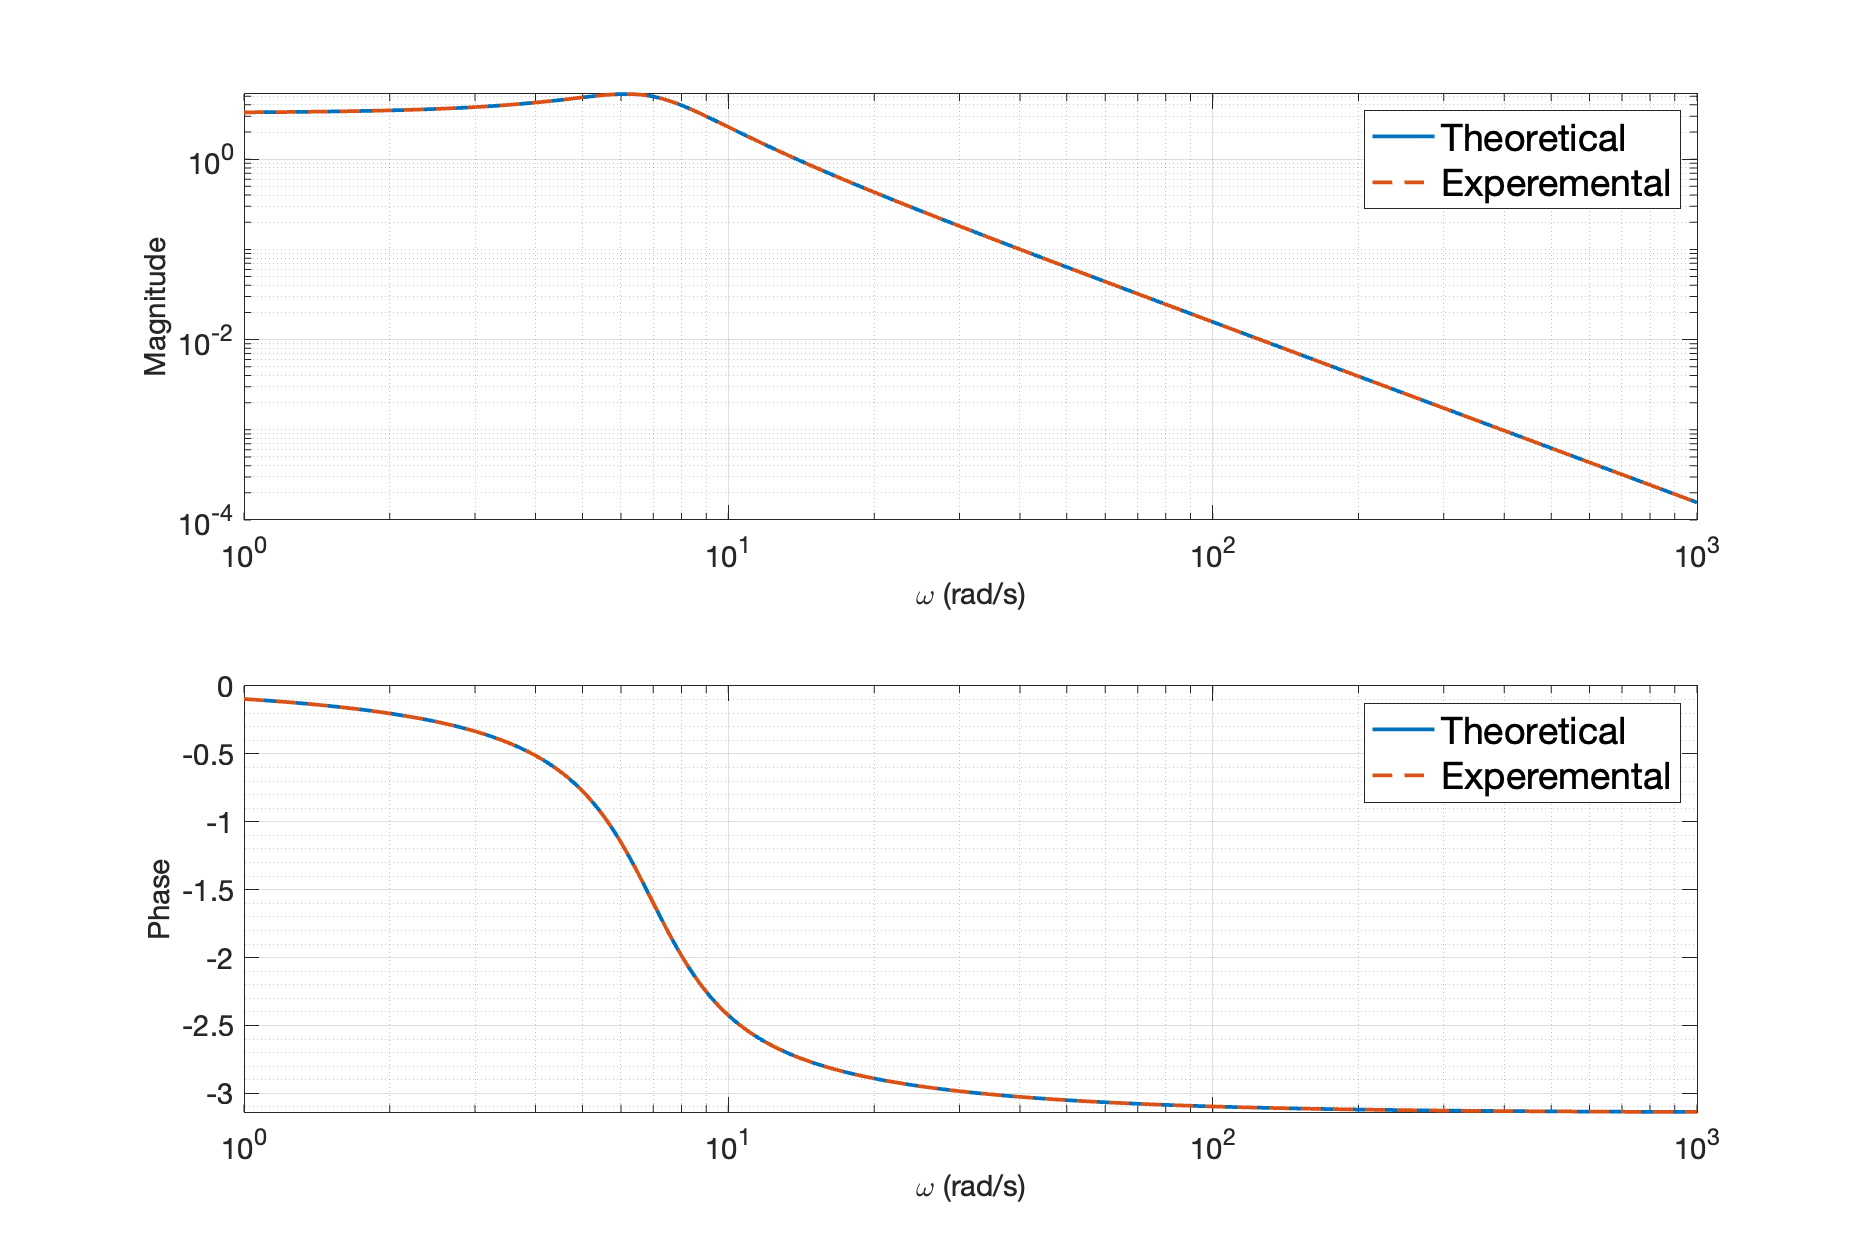
\includegraphics[width=\textwidth]{media/plots/task2_freq_resp_cmp_loglog.png}
    \caption{Сравнение логарифмической АЧХ двигателя постоянного тока 2.0}
    \label{fig:task2_freq_resp_cmp_loglog}
\end{figure}

